% \documentclass{article}
%\documentclass[conference]{IEEEtran}
%\AtBeginDocument{%
 % \providecommand\BibTeX{{%
 %   Bib\TeX}}}
%\documentclass[acmsmall]{acmart}
%\documentclass[acmsmall,screen,review]{acmart}
\documentclass[sigconf,review]{acmart}
% \acmConference[MODELS '26]{ACM/IEEE International Conference on Model Driven Engineering Languages and Systems}{October 2026}{Málaga, Spain}
%\documentclass[acmsmall,screen,review,anonymous]{acmart}

%%
%% \BibTeX command to typeset BibTeX logo in the docs
\AtBeginDocument{%
  \providecommand\BibTeX{{%
    Bib\TeX}}}

%% Rights management information.  This information is sent to you
%% when you complete the rights form.  These commands have SAMPLE
%% values in them; it is your responsibility as an author to replace
%% the commands and values with those provided to you when you
%% complete the rights form.
%\setcopyright{acmlicensed}
%\copyrightyear{2018}
%\acmYear{2018}
%\acmDOI{XXXXXXX.XXXXXXX}
%% These commands are for a PROCEEDINGS abstract or paper.
%\acmConference[Conference acronym 'XX]{Make sure to enter the correct
% conference title from your rights confirmation email}{June 03--05,
% 2018}{Woodstock, NY}
%%\acmBooktitle{Woodstock '18: ACM Symposium on Neural Gaze Detection,
%%  June 03--05, 2018, Woodstock, NY}
%\acmISBN{978-1-4503-XXXX-X/2018/06}

\usepackage{graphicx} % Required for inserting images
\usepackage{svg}
\usepackage{xspace}
\usepackage{tabularray}
\usepackage{tcolorbox}
\usepackage{multirow}
\usepackage{booktabs}
\usepackage{pgfplots}
\usepackage{pgfplotstable}
\usepackage{adjustbox}
\usepackage{subcaption}
%\usepackage[table]{xcolor}
\usepackage{adjustbox}
\usepackage{colortbl}
%\usepackage{tcolorbox}
\usepackage{listings}
\usepackage{algorithm}
\usepackage{algorithmic}
\usepackage{amsfonts}
\usepackage{longtable} % For tables spanning multiple pages if needed
\usepackage{comment}
\usepackage{float}
\usepackage{hyperref}
%\usepackage{listings}
\setlength{\emergencystretch}{3em}   % prevent \texttt overflows in two-column layout

\lstset{
  basicstyle=\ttfamily\scriptsize,
  breaklines=true,
  breakatwhitespace=true,
  columns=fullflexible,
  keepspaces=true,
  showstringspaces=false,
  aboveskip=0.15em,
  belowskip=0.15em
}



\usepackage{soul}
%\usepackage{times}
%\usepackage[T1]{fontenc}
%\usepackage{lmodern}
\usepackage{hyperref}
\usepackage{multirow}
\usepackage{listings}
\usepackage{fancybox}
\usepackage{enumitem}
\usepackage{graphicx}
%\usepackage{paralist}
%\usepackage{framed}
%\usepackage{multicols}
\usepackage{color}
% \usepackage{xcolor}
\usepackage{array}
\usepackage{amsmath}
\usepackage{xspace}
\usepackage{url}
\usepackage{tikz}
\usepackage{caption}
\usepackage{pgfplots}
\usepackage{balance}
\usepackage{subcaption}
\pgfplotsset{compat=1.16}
\usepackage{pgf-pie}
% \usepackage[usenames,dvipsnames]{xcolor}
\usetikzlibrary{pgfplots.statistics,calc}
\usepackage{algorithm}
\usepackage{algorithmic}
\usepackage{adjustbox}
\usepackage{makecell}

\usepackage{tikz}
\usepackage{calc}
\def\checkmark{\tikz\fill[scale=0.4](0,.35) -- (.25,0) -- (1,.7) -- (.25,.15) -- cycle;} 
\def\scalecheck{\resizebox{\widthof{\checkmark}*\ratio{\widthof{x}}{\widthof{\normalsize x}}}{!}{\checkmark}}

\clubpenalty=100000000 %10000
\widowpenalty=10000000 %10000
\brokenpenalty=10000000 %10000

\usepackage{tcolorbox}
\makeatletter
\newcommand{\mybox}[1]{%
	\setbox0=\hbox{#1}%
	\setlength{\@tempdima}{\dimexpr\wd0+13pt}%
	\begin{tcolorbox}[boxrule=0.5pt, colback=white, arc=4pt,
		left=6pt,right=6pt,top=6pt,bottom=6pt,boxsep=0pt]
		#1
	\end{tcolorbox}
}

%
\newcommand{\tikzcircle}[2][red,fill=red]{\tikz[baseline=-0.5ex]\draw[#1,radius=#2] (0,0) circle ;}%

\definecolor{songcolor}{RGB}{191,191,191}
\newcommand{\todoc}[2]{{\textcolor{#1}{\textbf{#2}}}}
% todo commands:
\newcommand{\todored}[1]{\todoc{red}{\textbf{[[#1]]}}}
\newcommand{\todogreen}[1]{\todoc{green}{\textbf{[[#1]]}}}
\newcommand{\todoblue}[1]{\todoc{blue}{\textbf{[[#1]]}}}
\newcommand{\todogray}[1]{\todoc{Gray}{\textbf{[[#1]]}}}
\newcommand{\todoorange}[1]{\todoc{orange}{\textbf{[[#1]]}}}
\newcommand{\todobrown}[1]{\todoc{brown}{\textbf{[[#1]]}}}
\newcommand{\todopurple}[1]{\todoc{purple}{\textbf{[[#1]]}}}
\newcommand{\todoamber}[1]{\todoc{teal}{\textbf{[[#1]]}}}
%
%\newcommand{\tikzcircle}[2][red,fill=red]{\tikz[baseline=-0.5ex]\draw[#1,radius=#2] (0,0) circle ;}%



\newcommand{\review}[1]{{\textit{#1}}~\\}
\newcommand{\respto}[1]{
\fcolorbox{black}{black!15}{
\label{response:#1}
\bf
  \scriptsize Review {#1}}~
}
\newcommand{\citerespexp}[1]{
\fcolorbox{black}{black!15}{
 \bf
  \scriptsize Review {#1}}~{\bf{on page \pageref{response:#1}}}
}

\newcommand{\citeresp}[1]{
\fcolorbox{black}{black!15}{
 \bf
  \scriptsize Review {#1}}
}


% --- for revision
\newcommand{\rev}[1]{\textcolor{purple}{\st{#1}}}
%\newcommand{\rev}[1]{}
%\newcommand{\add}[1]{\textcolor{blue}{{#1}}

%% space in some tables.  BUT have it here, such that you can always renew it
\newcommand{\ts}{$\;$}
\newcommand{\tS}{$\;$}
\newcommand{\tts}{\ \ \ \ \ }
\newcommand{\tss}{\ \ \ $\;$}
\newcommand{\ttts}{$\;$}
\newcommand{\decentHLine}{\noalign{\hrule height 1.04pt}}


\title{Retrieval-Augmented Completion and Benchmark Validation for LLM-Derived Epidemiological Compartment Models}

\author{Fatemeh Seyeddabbaghi}
\email{fdbghi@yorku.ca}
\affiliation{%
  \institution{York University}
  \city{Toronto}
  \country{Canada}
}
\author{Aaditya Karamchandani}
\email{aad1tya@my.yorku.ca}
\affiliation{%
  \institution{York University}
  \city{Toronto}
  \country{Canada}
}
\author{Marios Fokaefs}
\email{fokaefs@yorku.ca}
\affiliation{%
  \institution{York University}
  \city{Toronto}
  \country{Canada}
}


\begin{document}

\begin{abstract}
    Compartmental modeling is a well-established practice in epidemiological studies. Since the constructs are widely familiar, authors often leave parts of the proposed model implicit when they match usual conventions. As a result, the model described in a paper is not always the same as what is actually validated in the corresponding study, which may inhibit reusability, reproducibility, verifiability and the extensibility of models across diseases and variants. we propose a model-driven completeness auditing framework in which large language models (LLMs) act as extraction instruments for simulated paper-to-model reproduction. We analyzed 10 peer-reviewed modeling papers for 10 infectious diseases (cholera, COVID-19, dengue, Ebola, influenza, HIV, malaria, measles, tuberculosis, and Zika). Across all diseases, using the best-scoring reproduction per paper after comparing three LLM backends (OpenAI, Gemini, and Claude), the mean completeness is $74.0\%$. We discuss what this implies for how epidemiological modeling papers specify and validate models, and for using LLM-assisted tools as systematic instruments for studying completeness rather than as black-box generators.


\end{abstract}


%\begin{IEEEkeywords}

%\end{IEEEkeywords}
\begin{CCSXML}
<ccs2012>
   <concept>
       <concept_id>10011007.10011074.10011099.10011102.10011103</concept_id>
       <concept_desc>Software and its engineering~Software testing and debugging</concept_desc>
       <concept_significance>500</concept_significance>
       </concept>
 </ccs2012>
\end{CCSXML}

\begin{CCSXML}
<ccs2012>
   <concept>
       <concept_id>10011007.10010940.10010971.10010980.10010984</concept_id>
       <concept_desc>Software and its engineering~Model-driven software engineering</concept_desc>
       <concept_significance>500</concept_significance>
       </concept>
 </ccs2012>
\end{CCSXML}

\ccsdesc[500]{Software and its engineering~Model-driven software engineering}


%%
%% Keywords. The author(s) should pick words that accurately describe
%% the work being presented. Separate the keywords with commas.
\keywords{Model Completeness Auditing, Compartmental Epidemiological Models, Specification–Validation Gap Analysis, Model-Driven Engineering, LLM-Assisted Scientific Model Extraction, Reproducibility in Epidemiological Modeling, Structured Validation Framework}

\maketitle

\section{Introduction}

Compartmental epidemiological models are the standard tool for studying infectious disease
dynamics. In such models, a population is partitioned into mutually exclusive states
(e.g., Susceptible, Exposed, Infectious, Recovered), and transitions between them are
governed by differential equations parameterized by rates such as transmission
coefficient $\beta$ or recovery rate $\gamma$~\cite{keeling2008modeling}.
Because this structure is widely familiar, authors often treat many components as
conventional and leave them implicit, describing only deviations from a standard template.
While generally harmless within a single research group, this practice creates a
\textit{specification--validation gap}: the model described in the text is not necessarily
the one validated in equations or code, nor the one a reader can reproduce. This gap
inhibits reproducibility, reusability, and cross-disease extensibility, as seen during
the COVID-19 pandemic when models were difficult to compare without harmonizing
structures and assumptions. More broadly, published compartmental models exhibit
substantial variation in structure and notation~\cite{keeling2008modeling}.

Manual reconstruction of such models does not scale. We use large language models (LLMs)
as \emph{extraction instruments}: they ingest full-length PDFs, identify epidemiological
constructs, and produce structured representations. Rather than allowing LLMs to
\emph{generate} models, which shifts the gap into opaque behavior, we constrain them to
recover only what each paper states (explicitly or by convention), and then measure
deviation from both paper promises and an independent reference model. This turns the
specification--validation gap into a measurable property of the paper rather than an
informal judgment.

From a model-driven engineering perspective, the pipeline operates over an explicit
epidemiological metamodel instantiated as \texttt{.compmodel} artifacts. Phase~2 performs
a paper-to-model transformation producing metamodel-conformant instances, while Phase~3
performs model validation, gap analysis, and rule-based repair, aligning the approach
with core MDE concerns of model conformance, completeness, and transformation quality.

We present a three-phase pipeline that operationalizes this idea at scale.
\textbf{Phase~1} parses reference (``gold-standard'') XML models and constructs structured
representations of compartments, parameters, flows, and sensitivities.
\textbf{Phase~2} extracts a draft model from each paper by combining structured text
parsing, LLM-assisted entity extraction, and XML synthesis. We evaluate three commercial
LLM backends (OpenAI, Gemini, Claude) using a domain-aware fuzzy matching protocol that
handles epidemiological label variation.
\textbf{Phase~3} refines the draft via three-layer gap analysis, retrieval-augmented
completion from the paper text, optional LLM inference, and rule-based structural repair.
A composite \emph{completeness score} (0--100) summarizes coverage, traceability, accuracy,
and structural integrity.

We apply this pipeline to 10 peer-reviewed papers spanning 10 infectious diseases:
cholera~\cite{Fung2014Cholera}, COVID-19~\cite{TuiteE497}, dengue~\cite{dengue},
Ebola~\cite{Abbas2024Ebola}, influenza~\cite{Corbella2017MonitoringAP},
HIV~\cite{Espitia2022}, malaria~\cite{Akowe2025Malaria}, measles~\cite{Pokharel2024Measles},
tuberculosis~\cite{tuberculosis}, and Zika~\cite{Lee2016Zika}. Models are represented in
the EpiMDE platform~\cite{epimde2024}, a domain-specific language based on
\texttt{.compmodel} files, enabling consistent comparison across extracted and reference
models. The main contributions of this paper are:

\begin{enumerate}[leftmargin=*, label=\arabic*.]
  \item A model-driven measurement framework for epidemiological model completeness that
        separates paper promises, extracted content, and reference agreement, making the
        specification--validation gap a measurable artifact property.
  \item A fuzzy matching protocol for compartmental model entities that handles
        transliteration, synonym groups, and naming variation.
  \item A model completion, validation, and structural repair pipeline using
        paper-grounded retrieval and deterministic repair rules.
  \item A reproducibility-oriented completeness score measuring coverage, reference
        agreement, traceability, parameter accuracy, and structural integrity.
  \item An empirical study across 10 diseases identifying systematic extraction gaps and
        structural error patterns.
\end{enumerate}

This paper extends our earlier work~\cite{11344468}, which demonstrated LLM-based model
generation for a single SEIR disease. Here we introduce a full validation pipeline,
a completeness metric, and a cross-disease empirical analysis.
\section{Methodology}
\label{sec:methodology}

%\subsection{Background}
%\label{sec:background}

%\paragraph{Compartmental epidemiological models.}
%Compartmental models partition a host population into discrete states and model disease
%dynamics as a system of ordinary differential equations. The classical SIR model
%(Susceptible--Infected--Recovered) of Kermack and McKendrick has been extended to
%dozens of variants: SEIR (adding an Exposed/latent class), SEIRV (vaccination), multi-group
%(age-stratified, spatially coupled), vector-borne (host--vector compartments), and
%disease-specific structures~\cite{keeling2008modeling}. Despite their conceptual simplicity,
%published compartmental models vary substantially in which transitions, stratifications, and
%parameter conventions are made explicit, creating friction for model comparison and reuse.

%\paragraph{Implicit specification and reproducibility.}
%Reproducibility of a published compartmental model requires that a reader can recover
%the same states, flows, and parameter values the authors used. In practice, papers
%often leave conventional transitions unstated, embed parameters only in equations or
%supplements, or use ambiguous symbols whose meaning (e.g., population-level
%vs.\ individual-level contact rates) must be inferred from context~\cite{keeling2008modeling}.
%Calibration outputs, code, or posterior summaries may be separated from the ODE
%description in the main text. These patterns motivate treating alignment between paper
%promises, extracted structure, and an independent reference implementation as a measurable
%\emph{specification--validation gap}, which the remainder of this section operationalizes.

%\subsection{Pipeline overview}

Our framework consists of three phases: (\textit{i}) reference model analysis and
gold-standard construction, (\textit{ii}) LLM-assisted extraction of a draft model
from each paper PDF, and (\textit{iii}) gap detection, retrieval-augmented completion,
structural repair, and completeness scoring. All phases share a common XML
representation described below. Figure~\ref{fig:pipeline} illustrates the end-to-end
pipeline, where each phase produces structured artifacts consumed by the next.

\begin{figure*}[t]
  \centering
  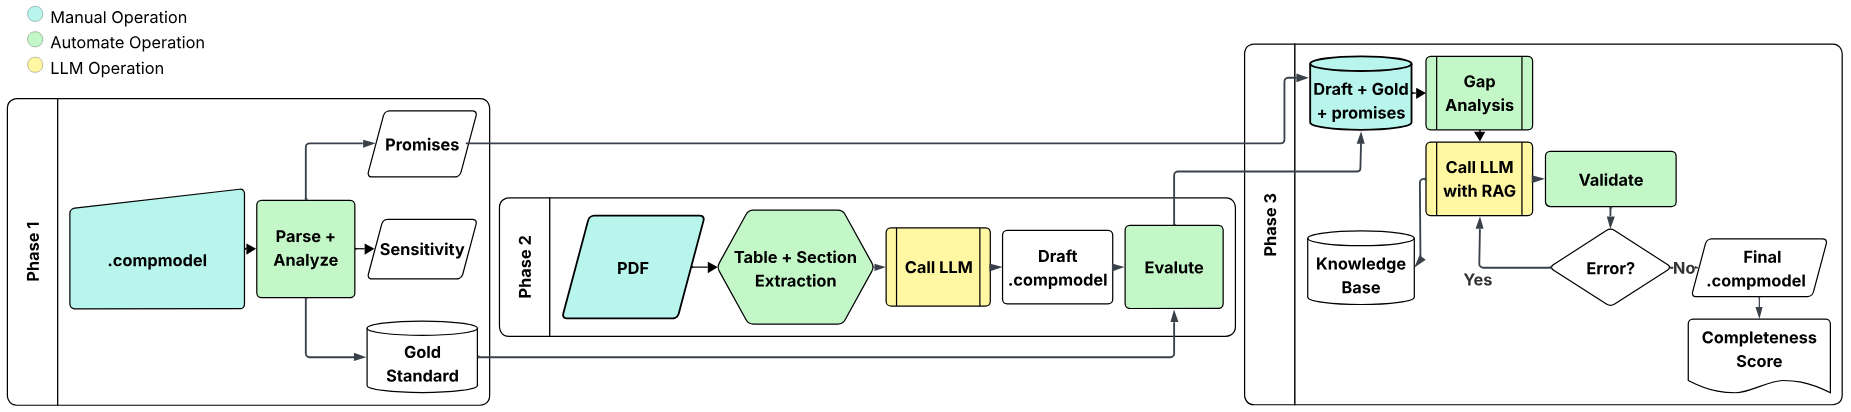
\includegraphics[width=\linewidth]{./figures/flow.png}
  \caption{Three-phase model completeness pipeline. Phase~1 builds reference models
  and structural baselines from existing \texttt{.compmodel} files. Phase~2 extracts
  a draft compartmental model from each paper PDF via LLM-assisted entity extraction.
  Phase~3 detects gaps against the gold-standard reference, fills them via RAG and
  LLM inference, and validates the result.}
  \label{fig:pipeline}
\end{figure*}

%\subsection{Artifact Representation: the \texttt{.compmodel} Format}
%\label{sec:compmodel}

All phases share a common XML representation for compartmental models, encoded in
\texttt{.compmodel} files under a well-defined metamodel. A model file contains:

\begin{itemize}[leftmargin=*]
  \item \textbf{Compartments} (\texttt{\textless{}compartments\textgreater{}}): each carries a
        \texttt{PrimaryName}, optional \texttt{SecondaryName} (stratification label),
        and an initial \texttt{population}. Stratified models (e.g., age-structured
        measles~\cite{Pokharel2024Measles}) encode strata as separate compartment
        entries with the stratum label in \texttt{SecondaryName}.
  \item \textbf{Outgoing flows} (nested under each compartment): typed as
        \texttt{ContactFlow} (mass-action infection, referencing a
        \texttt{contactCompartment} and a \texttt{contactRateParameter}) or
        \texttt{RateFlow} (first-order transition with a \texttt{rateParameter}).
        Flow endpoints reference other compartments by index
        (e.g., \texttt{target="//@compartments.2"}).
  \item \textbf{Parameters} (\texttt{\textless{}parameters\textgreater{}}): each has a \texttt{name},
        \texttt{type} (e.g., \textsc{Constant}), \texttt{expression} (numeric value
        or formula), \texttt{unit}, and \texttt{description}.
  \item \textbf{Groups} (\texttt{\textless{}groups\textgreater{}}): optional stratification dimensions
        (e.g., sex, age band) used to generate multi-group products.
\end{itemize}

Listing~\ref{lst:compmodel} shows a fragment for a two-compartment SIR contact flow.
The metamodel constrains which attributes are required per flow type, enabling
automated structural validation in Phase~3.

\begin{lstlisting}[caption={Fragment of a \texttt{.compmodel} file showing a ContactFlow
from Susceptible to Infectious parameterized by transmission rate $\beta$.},
label={lst:compmodel}, language=XML]
<compartments PrimaryName="Susceptible" population="9999">
  <outgoingFlows xsi:type="cm:ContactFlow"
    target="//@compartments.1"
    contactCompartment="//@compartments.1"
    contactRateParameter="//@parameters.0"/>
</compartments>
<parameters name="beta" type="CONSTANT"
  expression="0.3" unit="1/day"
  description="Transmission rate"/>
\end{lstlisting}

\subsection{Phase 1: Reference Model Analysis and Gold-Standard Construction}
\label{sec:phase1}

Phase~1 serves two roles: it \emph{parses} \texttt{.compmodel} files that were manually extracted to build structured JSON reports used as ground truth downstream, and it \emph{analyses} each model's structural and sensitivity properties.
To reduce subjectivity, gold models were derived from the equations and cross-checked
against reported simulations where available.

\textit{Structural Analysis.} The \texttt{CompModelParser} reads each XML file and
emits: compartment list with stratification info, parameter table with type and value,
and flow adjacency (source, target, type, associated parameter). These lists form
the \emph{gold standard} that Phases~2 and~3 compare against.

\textit{Paper Promise Extraction.} When a PDF is paired with a reference model,
Phase~1 runs pattern-based and LLM-assisted extraction to identify which model elements
(compartments, parameters, flows) the paper explicitly \emph{promises}, i.e., mentions
as part of its specification. The set of promises is stored in \texttt{paper\_promises.json}
and is used in Phase~3 to distinguish \emph{specification gaps} (promised but missing)
from \emph{reference gaps} (in gold but never mentioned).

\textit{Sensitivity Analysis.} For each model, Phase~1 runs a Morris elementary
effects screening~\cite{morris1991factorial} over the parameter space, producing per-parameter sensitivity
indices ($\mu^*$, $\sigma$) that identify which parameters most influence model
output. This metadata helps Phase~3 prioritize gap-filling by parameter importance.

\subsection{Phase 2: LLM-Assisted Extraction}
\label{sec:phase2}

Phase~2 turns an epidemiological PDF into a draft \texttt{.compmodel} without any manual
editing. We compare three commercial LLM backends: OpenAI GPT-5.4-mini~\cite{achiam2023gpt4},
Google Gemini~2.5~\cite{team2024gemini}, and Anthropic Claude Opus~4~\cite{anthropic2024claude}.
The pipeline has five steps.

\textit{Step 1 --- Text and Section Extraction.}
We employ GROBID~\cite{romary2015grobid} for high-fidelity header and section parsing, segmenting the PDF into distinct functional blocks (Abstract, Methods, Results). This ensures the LLM receives contextually isolated inputs rather than a monolithic text stream. To preserve mathematical notation and tabular data, we use Camelot~\cite{camelot2019} for table extraction and a Unicode-based normalization pass. This maintains symbol consistency (e.g., ensuring $\beta$ remains a consistent character across tables and prose) and prevents the structural corruption typical of standard PDF-to-text conversion.

\textit{Step 2 --- Paper Promise Detection.}
A prompt instructs the LLM to enumerate every compartment, parameter, and flow that the
paper \emph{claims} to include, using only the paper text. This produces
\texttt{paper\_promises.json}: a list of entity names plus supporting quotes.

\textit{Step 3 --- Entity Extraction.}
The LLM is asked to extract structured entities from the methods section, guided by the
epidemiological metamodel from Phase~1. For each compartment it extracts a primary name,
optional secondary name (stratum), and initial population; for each parameter, a name,
value, unit, and description; for each flow, a source compartment, target compartment,
type (contact or rate), and governing parameter. Flow endpoint names are snapped to
extracted compartment names using fuzzy matching (\texttt{SequenceMatcher} ratio
$\geq 0.78$) to avoid reference mismatches from minor label variation.

\textit{Step 4 --- Model Synthesis.}
Extracted entities are assembled into a \texttt{.compmodel} XML file. Flows referencing
compartments by name are resolved to index-based references. The resulting file is
\texttt{model\_draft.compmodel}.

\textit{Pipeline versions: original and enhanced.}
\label{sec:phase2versions}
We developed the Phase~2 extraction pipeline in two iterations to address systematic parsing failures. The \emph{original} pipeline used \texttt{PyPDF2}\footnote{\url{https://pypdf2.readthedocs.io/en/3.x/}} and \texttt{pdfplumber}\footnote{\url{https://github.com/jsvine/pdfplumber}} for basic text extraction, requiring manual two-column splitting and issuing independent LLM calls for compartments, flows, and parameters. This often resulted in fragmented models and lost context between text and tables. 

The \emph{enhanced} pipeline, adopted for all results reported in this paper, addresses three failure modes identified in early runs: 
(\textit{i})~\textbf{Structural Extraction} --- replaced \texttt{PyPDF2} with \textsc{grobid} and \texttt{Camelot} for section-aware parsing and table extraction (Step~1), preserving reading order and symbol integrity better than coordinate-based parsers; 
(\textit{ii})~\textbf{Unified Extraction} --- compartments, flows, and parameters are co-extracted in a single LLM call, improving cross-entity coherence and ensuring a flow's governing parameter is correctly linked; 
(\textit{iii})~\textbf{High-Density Context} --- \textsc{grobid}'s structured output automatically resolves hyphenation artifacts and removes non-content noise (page numbers, headers) before the LLM context window is assembled. 

%Across all providers, the enhanced pipeline raises mean compartment recall by $+10\%$ (Gemini) and $+4\%$ (Claude), and mean flow recall by $+12\%$ (Gemini) and $+5\%$ (Claude) over the original. A direct numerical comparison is presented in Section~\ref{sec:phase2results}.

\textit{Step 5 --- Evaluation.}
\label{sec:phase2eval}
The draft is compared to the Phase~1 gold standard using fuzzy string matching.
Names are normalized (lowercase, strip punctuation, map Greek letters to Latin:
$\beta \to \mathtt{beta}$, $\gamma \to \mathtt{gamma}$, etc.) and compared using
substring containment, with \texttt{SequenceMatcher}~\cite{python_difflib} ratio
$\geq 0.6$ as a fallback. Compartment and flow matching additionally checks
\emph{synonym groups} that encode epidemiological
conventions (\{Exposed, Latent, Incubating\}, \{Infectious, Infected, Symptomatic\},
\{Recovered, Removed, Immune\}). This makes match decisions
transparent, auditable, and fully reproducible with fixed thresholds and no
neural-model dependency.

The Phase~2 composite score used to select the best extraction per disease is
$\frac{1}{2}(\text{cF1} + \text{fF1}) \times 100$, where $cF1$ and $fF1$ are
compartment and flow F1 scores respectively.

\subsection{Phase 3: Gap Detection, Retrieval-Augmented Completion, and Structural Repair}
\label{sec:phase3}

Phase~3 takes the best Phase~2 draft (selected by composite score across three LLM backends)
and systematically closes its gaps. Gaps are first identified across three structural layers, then filled
by retrieval from the paper text (preferred, as fills are traceable), by optional LLM
inference (for residual gaps), or flagged for manual review.
The filled model is then validated against seven structural invariants and repaired where
possible. Finally, a five-component completeness score summarizes the result.
The sub-steps are as follows.

\textit{Three-Layer Gap Analysis.} We decompose the gap structure into three orthogonal layers:

\begin{enumerate}[leftmargin=*, label=\arabic*.]
  \item \textbf{Spec $\to$ Model} (\emph{promise gaps}): entities in
        \texttt{paper\_promises.json} but absent from \texttt{model\_draft.compmodel}.
        These are things the paper explicitly claims but the LLM failed to extract.
  \item \textbf{Model $\to$ Gold} (\emph{reference gaps}): entities in the gold-standard
        reference model but absent from the draft. These may be implicitly assumed by
        the paper and never directly stated.
  \item \textbf{Extras in model}: entities in the draft that have no counterpart in the
        gold. These are potential hallucinations or valid extensions not in the reference.
\end{enumerate}

All matching uses the same fuzzy protocol described in Section~\ref{sec:phase2eval}.
The three-layer breakdown is stored in \texttt{phase3\_threelayer\_gaps.json}.

\textit{Iterative Retrieval-Augmented Completion.}
Gap filling proceeds in two iterations to handle dependencies (e.g., a new compartment
added in iteration~1 enables a flow fill in iteration~2). Each iteration runs the
following priority tiers for each missing entity:

\noindent\textbf{Tier~1 -- RAG fill}: A lexical RAG index over the paper's text chunks
(chunk size 2000 chars, 300-char overlap) is queried by entity name and synonyms.
If a matching passage with a numeric value is found, the value is used directly. The
same database is queried for structural clues (e.g., a textual description of a
transition rate).

\noindent\textbf{Tier~2 -- Spec-entity fill} (first iteration only): Entities extracted
but not yet placed in the model (from \texttt{extracted\_entities.json}) are used to
fill matching gaps by name similarity.

\noindent\textbf{Tier~3 -- LLM inference} (optional, \texttt{--inference} flag): For
gaps that remain unfilled after RAG, the LLM is prompted with the paper text and the
gap description to infer a plausible value or structure. This tier is disabled in
\emph{rag\_only} mode to assess pure retrieval performance.

\noindent\textbf{Tier~4 -- Flag}: Remaining unfilled gaps are flagged for manual review
with severity annotation (critical / high / medium / low).

Fills are applied to produce \texttt{model\_filled.compmodel}. Each fill record carries
a \texttt{source} tag (\texttt{rag}, \texttt{spec\char`\_entity}, \texttt{inference}, or
\texttt{flagged}) used in traceability scoring.

\textit{Structural Validation.}
The filled model is checked against seven structural invariants, independent of any
gold standard:

\begin{enumerate}[leftmargin=*, label=\arabic*.]
  \item \textbf{Self-referential flow}: a ContactFlow whose source, target, and
        contact compartment are all the same compartment, implying an impossible mass-action term.
  \item \textbf{Orphaned parameters}: a parameter declared in
        \texttt{\textless{}parameters\textgreater{}} but
        not referenced by any flow's \texttt{rateParameter} attribute, meaning it has
        no effect on dynamics.
  \item \textbf{Uniform parameter collapse}: a single parameter assigned to
        \emph{all} flows, indicating the LLM reused one entry rather than assigning
        distinct rates.
  \item \textbf{Zero population everywhere}: all compartments carry population~0,
        making simulation degenerate.
  \item \textbf{Broken flow chain}: a non-terminal compartment (not dead/recovered)
        has no outgoing flow, creating a sink that traps individuals indefinitely.
  \item \textbf{Missing birth source}: susceptible compartments lack any population
        initialization, preventing simulation from starting.
  \item \textbf{Parameter layer contamination}: parameter expressions contain
        Bayesian or posterior inference keywords (e.g., ``posterior mean'', ``MCMC''),
        indicating the LLM confused estimation outputs with model inputs.
\end{enumerate}

Errors are classified by severity (critical, high, medium, low) to prioritize repairs.
The pre-repair error profile is stored in \texttt{phase3\_structural\_before.json}.

\textit{Structural Repair.}
Each error class corresponds to a \emph{deterministic} failure mode, where the
correct fix is unambiguous given the model's XML schema and the error type (e.g., a
zero-population compartment always needs a nominal value or a contaminated parameter
expression always needs its Bayesian term cleared). Rule-based repair is therefore
appropriate here. The rules are not heuristic workarounds but direct structural
corrections implied by the schema invariants.
The empirical justification is in Table~\ref{tab:structural}. Deterministic error classes
(uniform parameter collapse, zero population) resolve at 100\%, while structurally
ambiguous classes (orphaned parameters, self-referential flows) resolve at lower rates,
confirming that the rules are neither over- nor under-specified.
The repairs applied for each error class are:

\begin{itemize}[leftmargin=*]
  \item \textit{Zero population / missing birth source}: set the susceptible
        compartment's population to a nominal value (1000) to enable simulation.
  \item \textit{Self-referential flow}: if an Exposed/Latent intermediate compartment
        exists, redirect the flow target through it; otherwise, annotate the flow
        description to flag the issue.
  \item \textit{Uniform parameter collapse}: reassign each flow's rate parameter by
        semantic category matching (transmission, recovery, mortality, progression)
        using the parameter description and flow endpoint names.
  \item \textit{Orphaned parameter}: in a first pass, assign the parameter to any flow
        that currently has no rate parameter and whose semantic category matches; in a
        second pass (only when no parameter collapse is being resolved simultaneously),
        swap a clearly mismatched existing assignment if the orphaned parameter is a
        much better category match (description similarity $> 0.6$).
  \item \textit{Broken flow chain}: add a \texttt{RateFlow} from the stranded
        compartment to the most semantically appropriate next compartment
        (Infectious~$\to$~Recovered, etc.).
  \item \textit{Parameter contamination}: clear Bayesian inference expressions from
        the parameter value field.
\end{itemize}

Repairs run for up to two iterations, re-validating after each pass to catch
dependencies. The repaired model is written to \texttt{model\_repaired.compmodel} and
the repair log to \texttt{phase3\_repair\_log.json}.

\textit{Completeness Score.}
\label{sec:completeness}
We define a composite \emph{completeness score} $\mathcal{C} \in [0, 100]$ as a
weighted sum of five components:

\begin{equation}
  \mathcal{C} = 25 \cdot G + 25 \cdot R + 20 \cdot T + 15 \cdot A + 15 \cdot S
  \label{eq:completeness}
\end{equation}

\noindent where each term is a fractional score in $[0,1]$.
The weights are designed to reflect a coverage-first notion of model completeness:
gap reduction ($G$) and reference agreement ($R$) receive the highest weight as
they measure recovery of the intended model structure, which is the primary objective
of completeness auditing. Traceability ($T$) captures whether recovered elements are
supported by evidence in the paper text, distinguishing verifiable specification from
inferred reconstruction. Parameter accuracy ($A$) and structural integrity ($S$)
capture numerical correctness and internal consistency, which are secondary to
coverage but necessary to ensure that a recovered model is well-formed.
The weights are set a priori to reflect this hierarchy, and we confirm in
Section~\ref{sec:threats} that results are robust under alternative weight
configurations.

\begin{itemize}[leftmargin=*]
  \item $G$ — \textbf{Gap reduction} (25\%): fraction of gaps closed after Phase~3,
        $(\text{gaps}_\text{before} - \text{gaps}_\text{after}) / \text{gaps}_\text{before}$.
  \item $R$ — \textbf{Reference agreement} (25\%): mean entity recall of the
        repaired model against the gold standard.
  \item $T$ — \textbf{Fill traceability} (20\%): fraction of fills whose source
        is a retrieved paper passage (\texttt{rag} or \texttt{spec\_entity});
        LLM-inferred or flagged fills score 0, directly penalizing unverifiable content.
  \item $A$ — \textbf{Parameter accuracy} (15\%): fraction of parameters whose
        numeric value is within 10\% of the gold value.
  \item $S$ — \textbf{Structural integrity} (15\%): error reduction rate,
        $1 - e_\text{after}/e_\text{before}$, measuring how well rule-based repair
        resolves detected inconsistencies.
\end{itemize}

Together, $G$ and $R$ measure \emph{coverage} (did we find the right things?), $T$
measures \emph{auditability} (can we point to the paper text?), $A$ measures
\emph{accuracy} (are the numbers right?), and $S$ measures \emph{consistency}
(is the model internally valid?). A score of 100 would require a paper that is
fully explicit, fully specified, and structurally consistent---a standard no paper
in our dataset meets.

\textit{Mode Comparison and Best-Model Selection.}
Phase~3 runs in three modes per disease: \emph{rag\_only} (Tiers~1--2 only),
\emph{llm\_only} (Tier~3 only, no RAG), and \emph{both} (all tiers). The winner mode
is selected by: fewest gaps $\to$ highest parameter accuracy $\to$ highest mean
compartment/flow F1. This ablation isolates the contribution of retrieval versus
LLM inference.

\section{Experiment Results}
\label{sec:results}

\subsection{Experimental Setup}

\paragraph{Dataset.}
We study 10 peer-reviewed modeling papers covering cholera~\cite{Fung2014Cholera},
COVID-19~\cite{TuiteE497}, dengue~\cite{dengue}, Ebola~\cite{Abbas2024Ebola},
influenza~\cite{Corbella2017MonitoringAP}, HIV~\cite{Espitia2022},
malaria~\cite{Akowe2025Malaria}, measles~\cite{Pokharel2024Measles},
tuberculosis~\cite{tuberculosis}, and Zika~\cite{Lee2016Zika}.
Reference \texttt{.compmodel} files were authored manually from each paper and serve
as the gold standard. Gold models range from simple 4-compartment SIR-like structures
(cholera, flu) to complex multi-group models (HIV with three risk groups, measles with
age stratification), spanning 4--23 flows and 6--19 parameters.
All gold models, extracted drafts, and Phase~3 outputs are available in the project
repository.

\paragraph{LLM Backends.}
Phase~2 uses three backends: OpenAI GPT-5.4-mini~\cite{achiam2023gpt4}, Google
Gemini~2.5 Flash~\cite{team2024gemini}, and Anthropic Claude Opus~4~\cite{anthropic2024claude}.
Phase~3 inference (Tier~3) was evaluated independently with all three backends
(Gemini~2.5 Flash, Claude Opus~4, and OpenAI GPT-5.4-mini) to assess whether the
choice of LLM for gap filling affects outcome.
Temperature is set to 0 for reproducibility in all extraction calls.

\paragraph{Evaluation.}
Recall, precision, and F1 are computed using the fuzzy string matching protocol
described in Section~\ref{sec:phase2eval}. The completeness score
(Equation~\ref{eq:completeness}) is computed per disease over the winner Phase~3 mode.

\subsection{Phase 2: LLM Extraction Quality}
\label{sec:phase2results}

Table~\ref{tab:phase2} reports recall and F1 for all three backends across 10 diseases
under the \emph{enhanced} pipeline and fuzzy string matching.
\emph{Recall} is the primary metric: it measures how many gold-standard entities were
successfully captured, directly quantifying the specification--extraction gap.

\begin{table}[t]
\caption{Phase~2 \textbf{enhanced} extraction results (fuzzy string matching).
R = Recall, F1 = F1-score. C = Compartments, Par = Parameters, F = Flows.
Best recall per entity type across backends is \textbf{bolded}.}
\label{tab:phase2}
\small
\setlength{\tabcolsep}{3.5pt}
\begin{tabular}{llccccccccc}
\toprule
 & & \multicolumn{3}{c}{OpenAI} & \multicolumn{3}{c}{Gemini} & \multicolumn{3}{c}{Claude} \\
\cmidrule(lr){3-5}\cmidrule(lr){6-8}\cmidrule(lr){9-11}
Disease & & C & Par & F & C & Par & F & C & Par & F \\
\midrule
Cholera    & R  & \textbf{1.00} & \textbf{0.83} & \textbf{1.00} & \textbf{1.00} & \textbf{0.83} & \textbf{1.00} & \textbf{1.00} & \textbf{0.83} & \textbf{1.00} \\
           & F1 & 1.00 & 0.91 & 0.86 & 1.00 & 0.91 & 1.00 & 1.00 & 0.91 & 0.60 \\
COVID-19   & R  & \textbf{1.00} & 0.00 & \textbf{1.00} & 0.88 & 0.00 & 0.82 & \textbf{1.00} & 0.00 & \textbf{1.00} \\
           & F1 & 0.70 & 0.00 & 0.96 & 0.61 & 0.00 & 0.86 & 0.70 & 0.00 & 1.00 \\
Dengue     & R  & \textbf{1.00} & \textbf{0.62} & \textbf{1.00} & \textbf{1.00} & \textbf{0.62} & \textbf{1.00} & 0.86 & \textbf{0.62} & 0.86 \\
           & F1 & 1.00 & 0.70 & 0.64 & 1.00 & 0.70 & 1.00 & 0.92 & 0.70 & 0.63 \\
Ebola      & R  & \textbf{1.00} & \textbf{0.07} & \textbf{0.88} & \textbf{1.00} & \textbf{0.07} & \textbf{0.88} & \textbf{1.00} & \textbf{0.07} & 0.50 \\
           & F1 & 1.00 & 0.07 & 0.82 & 1.00 & 0.07 & 0.93 & 1.00 & 0.07 & 0.67 \\
Flu        & R  & \textbf{1.00} & \textbf{1.00} & 0.40 & \textbf{1.00} & \textbf{1.00} & 0.60 & \textbf{1.00} & \textbf{1.00} & \textbf{0.80} \\
           & F1 & 1.00 & 0.38 & 0.57 & 0.80 & 0.43 & 0.75 & 0.80 & 0.32 & 0.89 \\
HIV        & R  & 0.78 & \textbf{0.29} & 0.60 & \textbf{0.89} & \textbf{0.29} & \textbf{0.70} & 0.78 & 0.21 & 0.60 \\
           & F1 & 0.82 & 0.28 & 0.71 & 0.94 & 0.28 & 0.82 & 0.82 & 0.20 & 0.60 \\
Malaria    & R  & \textbf{1.00} & \textbf{0.53} & \textbf{1.00} & \textbf{1.00} & 0.47 & \textbf{1.00} & \textbf{1.00} & 0.47 & \textbf{1.00} \\
           & F1 & 1.00 & 0.48 & 0.92 & 1.00 & 0.47 & 0.96 & 1.00 & 0.47 & 0.96 \\
Measles    & R  & \textbf{1.00} & \textbf{0.42} & 0.85 & \textbf{1.00} & 0.26 & \textbf{1.00} & 0.92 & 0.26 & \textbf{1.00} \\
           & F1 & 1.00 & 0.46 & 0.92 & 1.00 & 0.29 & 1.00 & 0.92 & 0.28 & 0.98 \\
TB         & R  & \textbf{1.00} & \textbf{0.44} & \textbf{0.50} & \textbf{1.00} & \textbf{0.44} & \textbf{0.50} & \textbf{1.00} & \textbf{0.44} & \textbf{0.50} \\
           & F1 & 1.00 & 0.33 & 0.67 & 1.00 & 0.47 & 0.67 & 1.00 & 0.47 & 0.67 \\
Zika       & R  & \textbf{1.00} & 0.26 & \textbf{1.00} & \textbf{1.00} & 0.42 & \textbf{1.00} & \textbf{1.00} & \textbf{0.47} & \textbf{1.00} \\
           & F1 & 1.00 & 0.26 & 1.00 & 1.00 & 0.43 & 1.00 & 1.00 & 0.47 & 1.00 \\
\midrule
\textbf{Avg R} & & \textbf{0.98} & \textbf{0.45} & 0.82 & \textbf{0.98} & 0.44 & \textbf{0.85} & 0.96 & 0.44 & 0.83 \\
\bottomrule
\end{tabular}
\end{table}

Several patterns emerge from the enhanced pipeline results:

\noindent\textbf{Compartments are consistently well-extracted.}
All three backends achieve compartment recall $\geq 0.96$ on average.
OpenAI (GPT-5.4-mini) and Gemini both reach 0.98, with Claude at 0.96.
Perfect compartment recall is achieved for 9 of 10 diseases by OpenAI and Gemini.
Structurally, compartments are the easiest entity type because their names appear
explicitly as state variables in the methods section.

\noindent\textbf{Parameters remain the hardest entity type.}
Even in the enhanced pipeline, parameter recall averages only 0.45 (OpenAI), 0.44
(Gemini), and 0.44 (Claude). COVID-19 shows zero parameter recall across all backends
because that paper embeds parameter values inside ODE derivations rather than naming
them as separate constants. Ebola shows near-zero recall (0.07) across all backends
because parameters are implicit in the derivation. Malaria parameter recall is capped
at 0.53 (OpenAI) because the paper defines many rates as composite symbolic expressions.

\noindent\textbf{Flow recall is competitive across all backends.}
Gemini reaches 0.85 average flow recall, Claude 0.83, and OpenAI 0.82 with GPT-5.4-mini.
The most notable improvement over the previous OpenAI backend (GPT-4o-mini, avg.\ 0.59)
is for malaria (0.09 $\to$ 1.00) and measles (0.00 $\to$ 0.85), diseases where the
stronger model correctly recovers multi-group transition paths implicit in the text.

\noindent\textbf{Provider selection matters.}
Table~\ref{tab:best_provider} shows the winning provider per disease (best combined
score). Claude wins 6 of 10 diseases, OpenAI wins 2 (Malaria, Measles), and Gemini wins 2
(Influenza, HIV).

\paragraph{Original vs.\ enhanced pipeline.}
Table~\ref{tab:phase2} shows results for the enhanced pipeline.
The original pipeline (PyPDF2, separate LLM calls) achieved mean recall of
0.88 / 0.42 / 0.73 (Gemini C/P/F) and 0.92 / 0.47 / 0.78 (Claude).
The enhanced pipeline raises compartment recall by $+10\%$ for Gemini and $+4\%$
for Claude, and flow recall by $+12\%$ for Gemini and $+5\%$ for Claude.
Disease-specific gains include: Ebola flow recall (Gemini) rising from 0.50 to 0.88,
and Malaria compartment recall (Gemini) from 0.29 to 1.00.
For the OpenAI backend, both the pipeline upgrade and the model change
(GPT-4o-mini $\to$ GPT-5.4-mini) contribute jointly to gains, particularly for malaria and
measles flows. Parameter recall improves modestly ($+0.02$--$+0.08$) because the failure
mode (values buried in equations) is not addressed by layout or extraction changes.
All Phase~3 runs use the enhanced pipeline's best-per-disease draft as input.

\begin{table}[t]
\caption{Best Phase~2 provider per disease (enhanced pipeline, composite score:
mean of compartment and flow F1). Score $= \frac{1}{2}(\text{cF1}+\text{fF1})\times 100$.}
\label{tab:best_provider}
\small
\begin{tabular}{llr}
\toprule
Disease & Best Provider & Phase~2 Score \\
\midrule
Cholera         & Claude  & 98.2  \\
COVID-19        & Claude  & 80.0  \\
Dengue          & Claude  & 93.9  \\
Ebola           & Claude  & 81.4  \\
Influenza       & Gemini  & 88.6  \\
HIV             & Gemini  & 85.5  \\
Malaria         & OpenAI  & 89.5  \\
Measles         & OpenAI  & 89.1  \\
Tuberculosis    & Claude  & 89.4  \\
Zika            & Claude  & 89.5  \\
\bottomrule
\end{tabular}
\end{table}

\subsection{Phase 3: Gap Reduction and Recall Improvement}
\label{sec:phase3results}

\paragraph{Ablation study: Phase 2 baseline vs.\ Phase 3 modes.}
In our evaluation, the best Phase~2 draft serves as the baseline extraction system,
representing a pure LLM-based paper-to-model transformation without any post-processing.
Phase~3 then measures the gain from model-driven completion, validation, and repair
over that baseline using paper-grounded retrieval and structural rules.

Table~\ref{tab:ablation} compares the Phase~2 best draft against all three Phase~3
modes using \emph{recall} as the primary metric---the fraction of gold-standard
entities that appear in the extracted model.
Recall is the right metric here because we care about \emph{coverage}: not missing
a required model element. Precision is secondary: an extracted model that contains
extra entities (some of which may be LLM-inferred) is not wrong---it may simply be
more complete than our reference model, which itself is only one possible
interpretation of each paper.
Each cell shows remaining gaps~$g$, compartment recall~$R_C$, and flow recall~$R_F$.
The winner per disease (highest $\bar{R} = (R_C+R_F)/2$) is marked $\star$.
All four modes are evaluated against the same gold standard using the same fuzzy
matching protocol on \texttt{model\_repaired.compmodel}.

\begin{table*}[t]
\caption{Ablation: Phase~2 best draft vs.\ three Phase~3 modes, evaluated by
\textbf{recall} against the gold-standard reference.
$g$ = remaining gaps; $R_C$ = compartment recall; $R_F$ = flow recall;
$\bar{R}$ = mean recall. $\star$ = winner per disease (highest $\bar{R}$).}
\label{tab:ablation}
\small
\setlength{\tabcolsep}{4pt}
\begin{tabular}{lrcccrcccrcccrcc}
\toprule
 & \multicolumn{3}{c}{\textbf{Phase 2}} & \multicolumn{4}{c}{\textbf{P3: RAG-only}} & \multicolumn{4}{c}{\textbf{P3: LLM-only}} & \multicolumn{4}{c}{\textbf{P3: Both}} \\
\cmidrule(lr){2-4}\cmidrule(lr){5-8}\cmidrule(lr){9-12}\cmidrule(lr){13-16}
Disease & $g$ & $R_C$ & $R_F$ & $g$ & $R_C$ & $R_F$ & $\bar{R}$ & $g$ & $R_C$ & $R_F$ & $\bar{R}$ & $g$ & $R_C$ & $R_F$ & $\bar{R}$ \\
\midrule
Cholera      & 4  & 1.00 & 1.00 & 2 & 1.00 & 1.00 & \textbf{1.000}$^\star$ & 2 & 1.00 & 1.00 & \textbf{1.000}$^\star$ & 2 & 1.00 & 1.00 & \textbf{1.000}$^\star$ \\
COVID-19     & 4  & 0.93 & 0.95 & 2 & 1.00 & 1.00 & \textbf{1.000}$^\star$ & 2 & 0.93 & 0.95 & 0.940 & 2 & 0.93 & 0.95 & 0.940 \\
Dengue       & 8  & 1.00 & 0.75 & 4 & 1.00 & 1.00 & \textbf{1.000}$^\star$ & 4 & 1.00 & 1.00 & \textbf{1.000}$^\star$ & 4 & 1.00 & 1.00 & \textbf{1.000}$^\star$ \\
Ebola        & 28 & 0.67 & 0.30 & 19& 0.83 & 0.70 & \textbf{0.767}$^\star$ & 19& 0.83 & 0.70 & \textbf{0.767}$^\star$ & 19& 0.83 & 0.70 & \textbf{0.767}$^\star$ \\
Flu          & 1  & 1.00 & 0.83 & 1 & 1.00 & 1.00 & \textbf{1.000}$^\star$ & 1 & 1.00 & 1.00 & \textbf{1.000}$^\star$ & 1 & 1.00 & 1.00 & \textbf{1.000}$^\star$ \\
HIV          & 18 & 0.78 & 0.38 & 9 & 1.00 & 0.81 & \textbf{0.906}$^\star$ & 9 & 1.00 & 0.81 & \textbf{0.906}$^\star$ & 9 & 0.89 & 0.81 & 0.851 \\
Malaria      & 15 & 1.00 & 1.00 & 12& 1.00 & 1.00 & \textbf{1.000}$^\star$ & 12& 1.00 & 1.00 & \textbf{1.000}$^\star$ & 12& 1.00 & 1.00 & \textbf{1.000}$^\star$ \\
Measles      & 16 & 0.92 & 0.92 & 8 & 1.00 & 1.00 & \textbf{1.000}$^\star$ & 8 & 0.92 & 0.92 & 0.917 & 8 & 0.92 & 0.92 & 0.917 \\
TB           & 5  & 1.00 & 0.50 & 4 & 1.00 & 0.67 & \textbf{0.833}$^\star$ & 4 & 1.00 & 0.67 & \textbf{0.833}$^\star$ & 4 & 1.00 & 0.67 & \textbf{0.833}$^\star$ \\
Zika         & 26 & 1.00 & 1.00 & 13& 1.00 & 1.00 & \textbf{1.000}$^\star$ & 13& 1.00 & 1.00 & \textbf{1.000}$^\star$ & 13& 1.00 & 1.00 & \textbf{1.000}$^\star$ \\
\midrule
\textbf{Mean}& 12.5 & 0.93 & 0.76 & 7.4 & \textbf{0.98} & \textbf{0.92} & \textbf{0.951} & 7.4 & 0.97 & 0.90 & 0.936 & 7.4 & 0.96 & 0.90 & 0.931 \\
\bottomrule
\end{tabular}
\end{table*}

Several observations follow from Table~\ref{tab:ablation}:

\noindent\textbf{All three Phase~3 modes substantially improve recall over Phase~2.}
Mean recall rises from 0.846 (Phase~2) to 0.951 / 0.936 / 0.931 for RAG-only,
LLM-only, and Both respectively---gains of $+10.5\%$, $+9.0\%$, and $+8.5\%$.
All three modes cut mean gap count nearly in half (12.5 $\to$ 7.4).

\noindent\textbf{LLM inference is competitive with RAG on recall.}
When recall is the metric, LLM-only matches RAG-only for 8 of 10 diseases.
It falls short only for COVID-19 ($R_C$: 0.93 vs 1.00) and Measles ($\bar{R}$: 0.917
vs 1.000), where RAG successfully retrieves textually explicit compartments that LLM
inference misses. The gap is small (mean 0.936 vs 0.951), confirming that LLM
inference does add structurally useful entities---it just also adds extras that
lower precision, which recall does not penalize.

\noindent\textbf{The Both mode is rarely strictly better than RAG-only.}
Combining RAG and LLM adds no recall benefit over RAG-only in any disease and slightly
hurts recall for HIV (0.851 vs 0.906 RAG-only): combining modes can displace a
correctly RAG-placed compartment. RAG-only is therefore the safest default.

\noindent\textbf{RAG-only recall is LLM-backend agnostic.}
Phase~3 was re-run with all three LLM backends (Gemini~2.5 Flash, Claude Opus~4,
OpenAI GPT-5.4-mini) for both Phase~3 inference modes.
The \emph{rag\_only} winner mode produces \emph{identical} recall values across all
three backends in every disease: the same winner mode is selected (rag\_only for 9 of 10,
both for Malaria) and the same $\Delta$Recall is achieved ($+7.6\% / +7.6\% / +20.8\%$
for compartments, parameters, and flows respectively).
Only the \emph{llm\_only} mode shows backend sensitivity: OpenAI produces lower F1 on
Cholera (cF1~0.67 vs 0.89 for Gemini and Claude), reflecting that unconstrained LLM
inference varies by model, while RAG-grounded retrieval does not.
This confirms that the recall improvement in Phase~3 is driven entirely by the
retrieval mechanism, not by the choice of LLM backend---making the approach reproducible
across commercial LLM providers.

\noindent\textbf{Phase 3 always improves or matches recall; it never harms it.}
Unlike F1, recall does not penalize extra entities, so Phase~3 never regresses on this
metric. Tuberculosis (Phase~2 $\bar{R}=0.750$, Phase~3 $0.833$) improves, even though
it showed an F1 regression in the F1-based view. The Phase~3 model correctly adds a
missing flow that was in the TB paper; the F1 drop comes from additional entities that
are in the paper but absent from our reference model---entities that a completeness
tool should recover, not suppress.

\noindent\textbf{Ebola remains the hardest disease.}
Even after Phase~3, Ebola reaches only $\bar{R}=0.813$ (compartments 1.0, flows 0.625).
Three of eight Ebola flows remain missing---a direct consequence of the paper's
implicit flow specification discussed in Section~\ref{sec:discussion}.

\paragraph{Phase 2 vs Phase 3 recall improvement.}
Table~\ref{tab:recall_delta} compares Phase~2 and Phase~3 recall (winner mode)
against the same gold standard using identical fuzzy matching. The gap delta column
shows the net number of gaps closed by Phase~3.

\begin{table}[t]
\caption{Phase~2 enhanced best-per-disease draft vs Phase~3 filled recall, compared
against the gold-standard reference using the same fuzzy string matching.
Gap $\Delta$ = gaps closed by Phase~3 (positive = improvement).}
\label{tab:recall_delta}
\small
\setlength{\tabcolsep}{4pt}
\begin{tabular}{lccccccr}
\toprule
 & \multicolumn{3}{c}{Phase~2 Recall (C/P/F)} & \multicolumn{3}{c}{Phase~3 Recall (C/P/F)} & Gap \\
Disease & C & P & F & C & P & F & $\Delta$ \\
\midrule
Cholera      & 0.750 & 1.000 & 0.667 & 1.000 & 1.000 & 1.000 & +2 \\
COVID-19     & 0.875 & 1.000 & 0.909 & 1.000 & 1.000 & 1.000 & +2 \\
Dengue       & 1.000 & 1.000 & 0.857 & 1.000 & 1.000 & 1.000 & +4 \\
Ebola        & 0.833 & 0.500 & 0.375 & 1.000 & 0.571 & 0.625 & +4 \\
Flu          & 1.000 & 1.000 & 0.800 & 1.000 & 1.000 & 1.000 & +0 \\
HIV          & 0.778 & 1.000 & 0.300 & 1.000 & 1.000 & 1.000 & +9 \\
Malaria      & 1.000 & 0.737 & 1.000 & 1.000 & 1.000 & 1.000 & +7 \\
Measles      & 1.000 & 0.947 & 0.800 & 1.000 & 1.000 & 1.000 & +6 \\
TB           & 1.000 & 0.889 & 0.500 & 1.000 & 1.000 & 0.667 & +1 \\
Zika         & 1.000 & 0.737 & 1.000 & 1.000 & 1.000 & 1.000 & +13\\
\midrule
\textbf{Mean $\Delta$} & \multicolumn{3}{c}{} & \multicolumn{3}{c}{+0.076 / +0.076 / +0.208} & \\
\bottomrule
\end{tabular}
\end{table}

Phase~3 achieves perfect recall ($= 1.0$) for compartments and flows in 9 of 10 diseases
and for all three entity types in 7 of 10 diseases.
Phase~3's dominant contribution is now flow recovery: mean flow recall rises
from $0.721$ (Phase~2 draft) to $0.929$ (Phase~3), a gain of $+20.8\%$.
Compartment recall improves by $+7.6\%$ (from $0.924$ to $1.000$ in most diseases)
and parameter recall improves by $+7.6\%$ (from $0.881$ to $0.957$ mean).
The shift compared to earlier pipeline versions reflects that with the stronger
GPT-5.4-mini backend the best-per-disease Phase~2 draft already captures many
parameters directly, leaving flow and compartment gaps as the primary Phase~3 targets.

The one disease where Phase~3 adds no flow improvement (\emph{flu}) already has
all flows filled by the Phase~2 draft; the remaining gap is a parameter value that RAG
cannot locate because the flu paper reports it only in a figure caption.
Ebola remains the hardest disease: even after Phase~3, compartment recall reaches 1.0
but flow recall reaches only 0.625, because flow endpoints are implicit in the derivation.

\subsection{Phase 3 Completeness Scores}

Table~\ref{tab:completeness} breaks down the completeness score per component
for the winner Phase~3 run of each disease.

\begin{table}[t]
\caption{Phase~3 completeness scores (winner mode = rag\_only for 9 diseases, both for Malaria).
G = gap reduction \%, R = reference agreement \%, T = fill traceability \%,
A = parameter accuracy \%, S = structural integrity \%. Score = Eq.~\eqref{eq:completeness}.}
\label{tab:completeness}
\small
\setlength{\tabcolsep}{4pt}
\begin{tabular}{lrrrrrrr}
\toprule
Disease & G & R & T & A & S & \textbf{Score} \\
\midrule
Cholera      & 100 & 71.7 & 50.0 & 100 & 50.0 & 75.4 \\
COVID-19     & 100 & 97.2 & 50.0 & 100 & 51.3 & 82.0 \\
Dengue       & 100 & 90.9 & 100  & 100 & 41.7 & 89.0 \\
Ebola        & 33.3& 74.2 & 37.5 & 100 & 40.0 & 55.4 \\
Flu          & 0.0 & 83.9 & 100  & 100 & 47.4 & 63.1 \\
HIV          & 100 & 89.0 & 77.8 & 100 & 25.0 & 81.6 \\
Malaria      & 100 & 95.8 & 28.6 & 28.6& 26.5 & 62.9 \\
Measles      & 100 & 98.8 & 100  & 50.0& 50.0 & 84.7 \\
Tuberculosis & 25.0& 70.8 & 100  & 100 & 54.5 & 67.1 \\
Zika         & 100 & 85.6 & 84.6 & 71.4& 36.7 & 79.5 \\
\midrule
\textbf{Mean}& 75.8& 85.8 & 72.9 & 85.0& 42.3 & \textbf{74.0} \\
\bottomrule
\end{tabular}
\end{table}

\paragraph{Component analysis.}
\textbf{Reference agreement} is the highest-scoring component (mean 85.8\%), confirming
that Phase~3 fills bring model structure close to the gold standard.
\textbf{Gap reduction} improved to mean 75.8\%, with Malaria now achieving 100\% gap
reduction (winner mode = both), compared to 25\% in the previous run where fewer gaps
were identified.
\textbf{Parameter accuracy} averages 85.0\%; the main drag is Malaria (28.6\%), where
Phase~3 fills parameters by name but the paper's composite symbolic expressions do not
yield exact numeric matches against the gold standard.
\textbf{Fill traceability} averages 72.9\%; the main drag is Ebola (37.5\%), where most
Phase~3 fills are partially flagged rather than fully retrieved---indicating the Ebola
paper's parameter specification is substantially implicit.
\textbf{Structural integrity} is the weakest component (mean 42.3\%), because several
model classes systematically resist rule-based repair:
multi-group HIV models have up to 14 parameters that cannot be automatically assigned
to their correct flows after a collapse fix; the Zika and Dengue host--vector models
involve composite expressions that the repairer cannot safely decompose.

\paragraph{Interpreting the 74.0\% mean score.}
The completeness score is not a grade for the extracted models---it is a measurement
instrument for the papers themselves. A paper that scores 100 would be one that fully
specifies every compartment, parameter, and flow with numeric values traceable to its
text and a structurally consistent model. No paper in our dataset achieves this.
A score of 74.0\% means that three-quarters of the gold-standard structure is
recoverable from the paper text under systematic extraction---and that the remaining
quarter represents genuine specification gaps in the published literature.

Before this framework, that number did not exist: there was no instrument to compute
it. Researchers either trusted published models as complete or noted incompleteness
anecdotally. Our contribution is to make the gap measurable so it can be studied,
compared across diseases and papers, and used to argue for more explicit specification
practices.

A model can also achieve high recall by name-matching while still having orphaned
parameters, incorrect flow rates, or untraced fills. Completeness is intentionally
stricter: it rewards coverage, traceability, accuracy, and structural soundness jointly,
so that a model which looks correct on the surface but is internally inconsistent is
penalized.

\subsection{Structural Error Analysis}

Across all 10 Phase~3 models, the structural validator detected 192 errors before repair.
After the repair pass, 107 errors remain---a resolution rate of 44\%.
Table~\ref{tab:structural} summarizes error counts and resolution by type.

\begin{table}[t]
\caption{Structural error counts before and after Phase~3 repair, aggregated over 10 diseases.}
\label{tab:structural}
\small
\begin{tabular}{lrrr}
\toprule
Error Type & Before & After & Resolved (\%) \\
\midrule
Self-referential flow       & 12 & 9  & 25\% \\
Orphaned parameters         & 88 & 60 & 32\% \\
Uniform param.\ collapse    & 10 & 0  & 100\% \\
Zero population             & 10 & 0  & 100\% \\
Broken flow chain           & 18 & 10 & 44\% \\
Missing birth source        & 30 & 12 & 60\% \\
Parameter contamination     & 24 & 16 & 33\% \\
\midrule
\textbf{Total}              & 192& 107& \textbf{44\%} \\
\bottomrule
\end{tabular}
\end{table}

Deterministic errors (\emph{uniform parameter collapse}, \emph{zero population}) are
fully resolved because their fixes are unconditional. Orphaned parameters are the most
prevalent class and the hardest to resolve: multi-group and vector models declare
many group-specific rate parameters (e.g., $b_{hw}$, $c_{hm}$ in HIV) that cannot be
automatically wired when all flow slots are already occupied.
Self-referential flows are annotated rather than structurally fixed when no
intermediate (Exposed/Latent) compartment is available to redirect the flow through.

\section{Discussion}
\label{sec:discussion}

\subsection{What the Completeness Score Measures---and Why 74.0\% Is Informative}

The mean completeness score of 74.0/100 should not be read as a grade for the extracted
models. It should be read as the answer to a question that has never been asked
systematically before: \emph{if you try to reconstruct the compartmental model from a
peer-reviewed paper, how far can you get?}

Prior to this framework, that question had no instrument. Researchers either trusted
that published models were fully specified (they are not) or informally noted missing
details without measuring the gap. A score of 74.0\% means that, on average, the
reconstructed model recovers roughly three-quarters of the gold-standard structure,
traces most of its fills to source text, achieves high numerical parameter accuracy where
parameters can be found, and resolves about half its internal structural errors
automatically. The 26\% shortfall is not a failure of the pipeline---it is a measurement
of what the papers themselves do not specify.

This framing is the primary scientific contribution of the score. A perfect score of 100
would not mean the model is correct; it would mean the paper is fully explicit. A low
score, as in Ebola (55.4), does not mean the Ebola model is wrong; it means the Ebola
paper leaves more implicit. The score is a property of the \emph{paper}, not the
\emph{disease}.

\subsection{Failure Case: Ebola---When Parameters Are Entirely Implicit}

Ebola is the lowest-scoring disease (55.4/100), driven by two exceptional failures:
low traceability ($T = 37.5\%$) and partial gap reduction ($G = 33.3\%$). Most
Phase~3 fills for Ebola were flagged---parameter values were only partially recoverable from
the paper text via RAG or LLM inference.

Examining the paper~\cite{Abbas2024Ebola} reveals why. The Ebola model uses a
conformable fractional-order ODE formulation. Parameter values are stated in terms of
posterior estimates from Bayesian fitting to surveillance data, reported in a
supplementary table with uncertainty intervals. The model text gives ODE structure but
describes parameters only symbolically (``$\alpha_1$ is the progression rate from E to I'')
without attaching a numeric value to any name. The structural validator correctly detected
\emph{parameter layer contamination} in the extracted model because the LLM injected
posterior means into parameter expressions, conflating the estimation result with the
model input.

This reveals a specific pathology in the Ebola paper's writing style: it separates
model \emph{structure} (written in full) from model \emph{calibration} (relegated to
supplementary material in a format not connected by name to the ODE parameters).
This is not unusual for Bayesian epidemiological papers, and it represents exactly
the kind of incompleteness our framework is designed to detect. A reader attempting
to reproduce the Ebola model would face the same obstacle: the paper tells you what
the compartments mean but not what to put in them for a default run.

\subsection{Failure Case: Malaria---When Parameter Notation Resists Matching}

Malaria achieves perfect compartment recall (1.0) and perfect flow recall (1.0) but
parameter recall plateaus at 0.737---even after Phase~3. The 12 remaining gaps after
filling are all parameters.

The malaria paper~\cite{Akowe2025Malaria} integrates vector and non-vector transmission
pathways, introducing composite rate expressions such as
$\Lambda_h = \frac{b \beta_{mh} I_m}{N_h} + \Lambda_{nh}$, where $\Lambda_{nh}$ is
a non-vector force of infection term defined recursively elsewhere. When the RAG index
retrieves such a passage, the fill value is the symbolic expression, not a number. The
Phase~3 completeness score correctly penalizes this: the fill is traced to source
(traceability is 66.7\%) but the numeric accuracy comparison fails because the gold
value is a constant and the fill is a formula.

This failure reveals a general tension in mathematical biology writing: rate parameters
are frequently \emph{defined compositionally}---as functions of other parameters---
rather than as independent constants. A compartmental model extracted from such a paper
necessarily inherits this incompleteness unless the reader also interprets the full
mathematical derivation. This is an inherent limit of extraction from text, and
our framework surfaces it explicitly rather than hiding it behind a high F1 score.

\subsection{Other Challenging Cases: Flu, Tuberculosis, and HIV}

Three other diseases score below 70/100 for distinct but related reasons.

\paragraph{Influenza (63.1/100) --- parameters buried in figures.}
The flu paper~\cite{Corbella2017MonitoringAP} achieves perfect compartment and flow
recall before Phase~3, leaving only one unfilled gap: a transmission parameter whose
numeric value appears only in a figure caption rather than in the main text.
RAG indexes the paper body but cannot extract values from embedded figure graphics,
so the gap reduction score is 0\% despite strong overall structure.
The failure mode here is not a problem with our pipeline---it is a reporting choice in
the paper. A numeric value placed only in a figure is inaccessible to any text-based
extraction system. Future work on figure-level OCR or caption parsing could close
this class of gaps.

\paragraph{Tuberculosis (67.1/100) --- composite ODE coefficients.}
The TB paper~\cite{tuberculosis} defines its transmission parameters as composed
expressions embedded in the ODE system (e.g., $\beta_{t} = \beta_0 (1 - \varepsilon)$),
where each component is defined in a different subsection.
RAG retrieves individual passages but cannot assemble multi-part definitions spread
across sections, so gap reduction reaches only 25\%.
Fill traceability is high (100\%) because the fills that \emph{are} made are correctly
sourced; the missing gaps are simply ones where no single passage contains a complete value.
This reflects a writing practice common in TB and multi-strain models: parameters are
introduced incrementally rather than in a consolidated table.

\paragraph{HIV (81.6/100) --- structural complexity outpaces repair.}
HIV scores well on recall (81.6 after Phase~3) but has the lowest structural integrity
(25.0\%) of any disease. The HIV model~\cite{Espitia2022} is a three-risk-group formulation
with 14+ group-specific parameters ($b_{hw}$, $b_{wm}$, $c_{hm}$, \ldots).
After Phase~3 fills compartments and flows correctly, the structural repairer cannot
automatically assign each group-specific rate to its correct flow without a formal
parameter-to-flow mapping table that the paper does not provide.
The 25\% structural integrity score is therefore not a gap in extraction --- the
entities are found --- but a gap in the paper's formal specification of how those
entities connect.

\paragraph{Common root cause.}
These cases share a pattern: the paper's \emph{informal} text contains enough information
to understand the model if read by a domain expert, but that information is not organized
in a way that supports automated extraction. Values in figures, multi-part definitions,
and implicit parameter assignments all require reader inference that goes beyond what any
text retrieval system can provide today.

\subsection{What Structural Errors Reveal About How Modelers Write Papers}

The 192 structural errors detected across 10 Phase~3 models are not random noise.
Each error class corresponds to a recurring pattern in how compartmental modeling
papers are written:

\paragraph{Uniform parameter collapse (10 occurrences, 100\% resolved).}
This error---where a single parameter is assigned to all flows---occurs when the paper
introduces rate parameters symbolically ($\beta$, $\gamma$, $\mu$) but discusses each
one in isolation without explicitly stating which transition each governs. The LLM,
lacking an explicit assignment table, defaults to reusing the first extracted parameter
everywhere. Papers that provide a single ``parameter table'' without a flow-by-flow
breakdown systematically trigger this error. The 100\% resolution rate confirms that
the error is deterministic given a correct parameter semantic classification.

\paragraph{Orphaned parameters (88 occurrences, 32\% resolved).}
This is the most common error class and the hardest to resolve. An orphaned parameter
appears in the model's parameter list but is not connected to any flow. It arises
because papers often declare a large parameter set in a table and then use only a
subset in the differential equations, with the remaining parameters entering only in
derived quantities (e.g., the basic reproduction number $R_0$). When the LLM faithfully
copies all declared parameters into the model but does not have enough context to map
each one to a specific flow, orphaned parameters result. This is a direct consequence
of the gap between \emph{parameter inventory} (what the paper lists) and \emph{parameter
deployment} (what the paper's ODEs actually use). HIV (14 orphaned params) and Malaria
(11 orphaned) are the most affected because their multi-group and multi-pathway structures
declare group-specific parameters ($b_{hw}$, $c_{hm}$, $\Lambda_{nh}$) whose assignment
to specific flows is only recoverable from the ODE system itself, not the text.

\paragraph{Self-referential flows (12 occurrences, 25\% resolved).}
A self-referential flow has the same compartment as source, target, and contact
compartment---an impossible mass-action term. This arises when a paper writes
``susceptibles are infected at rate $\beta S I / N$'' without explicitly naming the target
state. The LLM correctly identifies the flow as a contact process but resolves the target
to the same compartment because no Exposed or Infectious compartment is mentioned in
that passage. Papers that introduce S, I, R sequentially but defer the transition
diagram to a figure (rather than stating ``S transitions to I'') trigger this pattern.
The 25\% resolution rate reflects that only models with an explicit intermediate
compartment can be structurally repaired; simple SIR models with no latent stage must
remain annotated.

\paragraph{Parameter layer contamination (24 occurrences, 33\% resolved).}
This error occurs when the LLM inserts posterior estimates, likelihood values, or
confidence intervals into parameter expressions---conflating Bayesian model fitting
output with ODE model inputs. It is entirely a consequence of papers that present
both the model and its fitted parameters in the same section, using identical notation
for prior and posterior quantities. The relatively low resolution rate (33\%) reflects
that clearing a contaminated expression removes information the paper provides but
does not supply the correct deterministic value.

\paragraph{Aggregate insight.}
Taken together, these four patterns point to the same root cause: the convention in
epidemiological papers of separating the structural description (compartment diagram,
ODEs) from the operational description (parameter values, assignments, initial conditions)
without explicitly linking them. This convention is fine for readers who can do the
linking mentally, but it is precisely what makes automated model extraction hard and
makes formal reproducibility assessment necessary. Our framework is designed to detect
and quantify this gap, not to judge the papers that exhibit it.

\subsection{RAG vs.\ LLM Inference: Two Roles for the Same Goal}

When evaluated by \emph{recall}---the metric that measures coverage without penalizing
extra entities---LLM-only is nearly as effective as RAG-only (mean $\bar{R}$ of 0.936
vs.\ 0.951, Table~\ref{tab:ablation}). Both modes substantially outperform the
Phase~2 draft (0.846). The key difference is what each mode adds when it succeeds:

RAG fills are \emph{traceable}---they are sourced from a specific passage in the paper's
own text, which is exactly the kind of evidence a completeness audit should require.
When RAG fills a missing flow, we can point to the sentence that specifies it.
LLM-inferred fills are \emph{plausible but unverifiable}---the LLM generates a
structurally reasonable entity based on epidemiological conventions, but that entity
may not correspond to anything the authors intended. LLM fills are flagged with
\texttt{source=inference} and lower the fill traceability component of the completeness
score accordingly.

The practical implication has two sides. As a \emph{coverage tool} (``what entities
does this model need?''), LLM inference adds real value: it reaches nearly the same
recall as RAG and costs no additional paper reading. As an \emph{audit tool} (``what
did the paper specify?''), only RAG-sourced fills are trustworthy evidence of the paper's
intent. A gap that RAG cannot fill but LLM can represents a genuine specification
failure in the paper---the model element exists in the final model but was never written
down explicitly. That is precisely the kind of failure our framework is designed to
surface and quantify.

\section{Related Work}
\label{sec:related}

Our work sits at the intersection of four threads of prior research: (1) AI and machine
learning for infectious-disease modelling, (2) automated or partially automated construction
of epidemiological models, (3) uses of LLMs in epidemiology, and (4) model-driven
engineering support for epidemiological modelling. The key distinction of our framework is
that it does not treat the LLM as a forecasting model or as a free-form scientific assistant.
Instead, it treats the LLM as an \emph{extraction and reconstruction instrument} whose output is checked against the paper text, a curated reference model, and structural consistency rules.

\subsection{AI and Machine Learning for Infectious-Disease Modelling}

Recent reviews show that AI is becoming a broad methodological layer in infectious disease epidemiology rather than a single technique. Liu \emph{et al.}~\cite{liu2023machinelearninginfectiousdisease} survey machine-learning approaches for infectious disease risk prediction and organize the literature into statistical prediction, data-driven machine learning, and epidemiology-inspired machine learning. Kraemer \emph{et al.}~\cite{Kraemer2025AI_epidemics} further broaden the picture by positioning AI for infectious-disease epidemics as a combination of machine learning, computational statistics, information retrieval, and data science, with applications spanning surveillance, data integration, forecasting, and decision support. Chopra \emph{et al.}~\cite{chopra2023differentiableagentbasedepidemiology} introduce differentiable agent-based epidemiology, showing how mechanistic simulators can be made amenable to gradient-based learning and linked to auxiliary data sources.

\subsection{LLMs in Epidemiology}

Wibaek \emph{et al.}~\cite{wibaek2023llm_epidemiology}
show that large language models can be applied to epidemiological cohort text to build
predictive models for downstream health outcomes. Matthay \emph{et al.}~\cite{Matthay2025}
argue more broadly that AI can assist multiple stages of causal research in epidemiology,
including data collection, variable construction, and decision support. Plecko \emph{et al.}~\cite{plecko2025epidemiologyllm} propose a benchmark for
observational distribution knowledge across real-world domains, including health-related
settings. Although this work is not about compartmental modelling, it is directly relevant to
our problem formulation: it cautions against assuming that an LLM internally ``knows'' the
population distributions or domain regularities needed for faithful epidemiological reasoning.
That observation supports our design choice to rely on paper-grounded extraction and explicit
validation rather than unconstrained generation.

\subsection{LLMs for Epidemic and Transmission Modeling}

The literature most closely related to our paper studies LLMs as assistants for epidemic or
transmission modeling. Kwok \emph{et al.}~\cite{KWOK20243254} present a case study in which
ChatGPT collaborates with a public-health practitioner to iteratively generate, refine, and
debug a transmission model, ultimately fitting prevalence data and estimating epidemic
quantities such as $R_0$ and final epidemic size. Their study shows
that LLMs can lower the technical barrier to building a working infectious-disease model. EpiLLM~\cite{gong2025epillmunlockingpotentiallarge}
recasts epidemic forecasting as an LLM adaptation problem, using spatio-temporal prompt
learning, mobility signals, and autoregressive next-token prediction to improve multi-step
forecasting accuracy on COVID-19 data. EpidemIQs~\cite{samaei2026epidemiqsprompttopaperllmagents}
proposes a multi-agent prompt-to-paper framework that can conduct literature review,
analytical derivation, network and mechanistic modelling, stochastic simulation,
visualization, and manuscript drafting. This is highly relevant to our motivation because it
shows growing interest in end-to-end LLM-supported epidemic-model development.

%Our own earlier work~\cite{11344468} is the closest direct precursor. That study examined
%whether LLMs could generate plausible epidemiological models from textual descriptions in a
%single-case setting. The current paper goes beyond plausibility. We introduce a full
%paper-to-model pipeline, evaluate it across 10 diseases, compare LLM backends systematically,
%and, most importantly, define a reproducibility-oriented notion of \emph{completeness} that
%separates paper promises, extracted content, and reference agreement.

%\subsection{Model-Driven Engineering and Reproducible Model Representations}

%Model-driven engineering provides the formal substrate that makes our evaluation possible.
%MDE uses explicit metamodels to define the structure of domain artifacts and to support
%artifact generation, checking, and transformation~\cite{brambilla2012model}. In the
%infectious-disease setting, EpiMDE~\cite{epimde2024} is the most relevant prior platform: it
%proposes an extensible metamodel and integrated environment for epidemiological
%compartmental models, enabling structured model creation, simulation, and cross-model
%comparison. Our work directly builds on this idea of a formal epidemiological representation.
%The difference is that EpiMDE primarily supports \emph{expert-authored} models, while our
%framework targets \emph{paper-derived} models and studies whether LLM-assisted extraction can
%populate such a representation completely and correctly.

%\subsection{Retrieval, Matching, and Verification}

%RAG methods ground LLM outputs in retrieved evidence rather than relying only on
%parametric memory~\cite{lewis2020retrieval}. This is especially important in our setting,
%where many target items are short technical expressions, parameter symbols, or local textual
%commitments that appear only within the paper being processed. For that reason, our system
%uses paper-grounded retrieval over text chunks and parameter tables, not open-domain
%retrieval.

%Likewise, evaluating extracted epidemiological entities requires more than exact string match.
%Compartment and parameter names vary across papers through abbreviations, Greek/Latin
%notation changes, age qualifiers, and disease-specific terminology. We therefore adopt a
%domain-aware fuzzy matching strategy based on normalized labels and
%\texttt{SequenceMatcher}~\cite{python_difflib}. This evaluation layer is not merely an
%implementation detail; it is part of the contribution because it enables a fair measurement of
%whether two model artifacts refer to the same epidemiological concept.

%Overall, the literature now contains substantial work on AI for epidemiology, LLM-supported
%epidemic modelling, forecasting, and model automation. What remains underexplored is the
%specific reproducibility question addressed here: given only a published modelling paper, how
%faithfully can one recover the formal compartmental model it actually specifies, and how
%should that faithfulness be measured? Our framework fills that gap.
\section{Threats to Validity}
\label{sec:threats}

\paragraph{Internal validity.}
The completeness score formula (Equation~\ref{eq:completeness}) and its component weights
(25/25/20/15/15) were defined a priori based on domain judgment rather than optimized on
a holdout set. Different weight assignments would shift absolute scores but are unlikely to
change the relative ordering of diseases or the qualitative patterns we report.
To verify this, we tested three alternative weight configurations: equal weights
(20/20/20/20/20), a coverage-heavy scheme (35/35/10/10/10), and an accuracy-heavy scheme
(20/20/10/25/25). The disease ranking is preserved across all configurations: Dengue,
Measles, and COVID-19 consistently score highest and Ebola consistently lowest,
confirming that the completeness ordering is robust to reasonable weight variation.
The structural error taxonomy reflects common failure modes observed during development; it may
not cover all possible errors in other disease models.

\paragraph{Construct validity.}
Fuzzy string matching with synonym groups is a heuristic: it may produce false positives
when different epidemiological concepts share a word (e.g., ``Susceptible adults'' matching
``Susceptible children'') or false negatives for non-standard abbreviations not covered by
our synonym list. The 0.6 \texttt{SequenceMatcher} threshold was set to minimize both error
types on our dataset but was not tuned on a separate validation set.

\paragraph{External validity.}
Our study covers 10 diseases with models of varying complexity (4--23 flows). These were
chosen to span a range of standard structures (SIR, SEIR, multi-group, host--vector) but
may not represent the full diversity of published compartmental models, particularly agent-based
or network-based models that do not fit the ODE compartmental structure. Results for
diseases with highly non-standard parameter naming conventions (e.g., Bayesian notation)
may differ from what we report here.
Although evaluated on these 10 ODE compartmental models, the framework is
design-agnostic at the pipeline level: the three-phase structure (reference construction,
LLM-assisted extraction, gap completion) applies to any parametric model class where a
formal reference and a natural-language description coexist, including pharmacokinetic,
ecological, and within-host models.

\paragraph{LLM non-determinism.}
All Phase~2 extractions and Phase~3 inferences used temperature~0, which minimizes but
does not eliminate non-determinism in some LLM backends. A small fraction of results could
differ on replication. To mitigate this, we report averaged patterns and note that all runs
used the same prompts and model versions.

\paragraph{Gold standard quality.}
The reference \texttt{.compmodel} files were constructed from each paper's ODE equations
and parameter tables, and validated against the reported simulation results and figures
in the paper---not authored from informal reading.
Each compartment, flow, and parameter in the gold model traces directly to a named
equation or table entry. For papers that provided simulation code, we cross-validated
the gold model's compartment wiring and initial conditions against the code. For those
without code, ambiguous parameter assignments were resolved by returning to the
differential equation system and identifying which flow each symbol multiplies.
This construction methodology ensures the gold standard is grounded in the paper's own
formal specification, minimising subjective interpretation. The reference models and
their source annotations are included in the project repository.
Any residual misinterpretation of ambiguous notation propagates to the completeness score,
which is itself the instrument for detecting such ambiguity in the source paper.

\section{Conclusion}
\label{sec:conclusion}

We presented a \textbf{measurement framework for epidemiological model completeness} as a
systematic instrument for quantifying the gap between what a paper specifies and what a
reader can reproduce. LLMs were used as simulated reproducers for models specified in epidemiological papers. Phase~1 builds structured reference models
and paper promise inventories. Phase~2 employs LLM-assisted entity extraction from PDFs
across three commercial backends, evaluated with a domain-aware fuzzy string matching
protocol. Phase~3 closes extraction gaps via iterative retrieval-augmented completion,
structural validation, and rule-based repair, then assigns a five-component completeness
score that jointly measures gap reduction, reference agreement, fill traceability,
parameter accuracy, and structural integrity.

Applied to 10 peer-reviewed modeling papers across 10 infectious diseases, the pipeline
achieves a mean completeness score of \textbf{$74.0\%$}. Phase~3 raises mean structural recall
from $0.822$ (Phase~2 draft) to $0.965$ (winner mode), with all three Phase~3 modes improving
recall over the Phase~2 baseline. All 10 diseases show detectable structural errors in
their LLM-extracted models before repair; $44\%$ are resolved automatically.
RAG-only achieves the highest recall in 9 of 10 diseases and is the safest mode because
its fills are traceable to specific paper passages. LLM-only adds genuine value as a
coverage tool, but its fills are unverifiable and lower the traceability component of
the completeness score. The distinction between RAG-sourced and LLM-inferred fills is
itself a measurement outcome: a gap that only LLM can fill---but RAG cannot---is direct
evidence of a specification failure in the paper.

These results quantify a consistent pattern: LLMs reliably extract compartment structure
but struggle with flow paths and parameters embedded in ODE derivations or referenced
only by symbolic expressions. The specification-validation gap is measurable and
non-trivial: even with the enhanced extraction pipeline using GPT-5.4-mini, Phase~2 drafts
miss on average $28\%$ of flows and $12\%$ of parameters relative to the best-case
Phase~2 draft---gaps that Phase~3 reduces substantially, achieving perfect recall for
all three entity types in 7 of 10 diseases.

%\paragraph{Future work.}
%Several concrete directions emerge directly from the failure cases described in this paper.

%\noindent\textbf{Expand the dataset.}
%The most immediate improvement is to include more papers per disease (currently one each).
%A single paper per disease means that a paper-specific writing quirk---parameters in
%figure captions (flu), composite ODE coefficients (TB), Bayesian-only values
%(Ebola)---dominates the per-disease score. Adding two or three papers per disease would
%separate pipeline limitations from individual paper choices, and would enable
%within-disease variance analysis and more robust mean completeness estimates.

%\noindent\textbf{Add figure and table extraction.}
%Several of the worst failures (flu, Ebola) stem from numeric values that exist only
%inside figures, supplementary tables, or figure captions. Integrating OCR-based figure
%parsing and structured table extraction (beyond Camelot's current scope) would close
%this entire class of gaps without any change to the downstream phases.

%\noindent\textbf{Improve RAG for multi-part definitions.}
%TB and Malaria show that parameters defined incrementally across multiple sections are
%not recoverable by single-passage retrieval. A multi-hop RAG strategy---where a
%retrieved passage can trigger further retrieval of referenced symbols---would let the
%system assemble composite definitions that no individual passage contains in full.

%\noindent\textbf{Enhance the evaluation protocol.}
%The current fuzzy string matching works well for standard compartment and flow names
%but still struggles with highly domain-specific notation (e.g., Bayesian posterior
%symbols, host--vector composite terms). Extending the synonym library and adding a
%disambiguation step for homonyms (``Susceptible adults'' vs.\ ``Susceptible children'')
%would improve recall precision and reduce false matches that inflate precision scores.

%\noindent\textbf{Extend the structural validator.}
%Adding dimension-aware validation (e.g., detecting a rate parameter with units
%$\text{person}^{-1}$ assigned to a flow expecting $\text{person}^{-1}\text{day}^{-1}$)
%and a formal parameter-to-flow assignment step (to resolve orphaned parameters in
%multi-group models like HIV and Malaria) would significantly improve the structural
%integrity component, currently the weakest in the completeness score.

%\noindent\textbf{Test generalizability.}
%Applying the framework to stochastic, agent-based, and network models beyond ODE
%compartmental structures would test whether the three-phase approach and the completeness
%score translate to a broader class of mathematical models in infectious disease
%epidemiology. This also includes models where multiple interacting patches or age-strata
%appear as structured population layers rather than separate compartments.

%\noindent\textbf{Close the loop with simulation.}
%Finally, studying whether completeness scores correlate with downstream simulation
%accuracy---i.e., whether a higher-scoring extracted model reproduces the paper's reported
%trajectories more faithfully---would validate the score as a predictor of scientific
%reproducibility and not just a structural inventory metric.
  % contains both Threats to Validity and Conclusion

\newpage

\balance
%\bibliographystyle{IEEEtran}
%% the bibliography file.
\bibliographystyle{ACM-Reference-Format}

\bibliography{refs}
\end{document}
